
After Bingo has been trained, it groups the best-performing equations into a Pareto front. In this graphical representation, the x-axis represents the complexity of each equation, while the y-axis signifies the fitness of each equation. Typically, models with lower complexity are more interpretable, but they may exhibit higher errors due to under-fitting. The Pareto front helps identify models that strike a balance between fitness and complexity.

The final SIF model can be selected in two ways. The first method involves selecting the equations for $f_w$, $M$, and $g$ individually and then combining them into a single SIF model. The alternative approach is to calculate all possible combinations of the candidate $f_w$, $M$, and $g$ equations to create a new Pareto front for the SIF models. This newly formed Pareto front is then used to choose the final model. Both of these methods aim to minimize complexity while ensuring fitness is at least as good as the equations from \cite{RNeqnsbook}.


Multiple equations were chosen for both of the model selection methods. This was done to create multiple comparison points between GPSR and the Raju-Newman equations. To lower the number of equations presented for the individual selection process the same $f_w$ (eqn \ref{eqn:Bingo_fw_common} and $M$ (eqn \ref{eqn:Bingo_M_common}) equations are used for all four models with only the $g$ equation changing.  

\begin{equation} \label{eqn:Bingo_fw_common}
    f_w = \sqrt{\frac{\sqrt{\frac{a}{t} + \cos\left(\frac{a}{t}\right)}}{\cos\left(\frac{c}{b}\right)}}
\end{equation}

\begin{equation} \label{eqn:Bingo_M_common}
    M = 1 + 0.06\left(\frac{a}{t}\right)^2\left(\frac{a}{c} - 1 \right) + \left(1 - \frac{c}{a} \right) \left(0.0069 \frac{c}{a} - 0.28 \frac{a}{t} \right)
\end{equation}


Using equation \ref{eqn:Bingo_g_matching_error} for $g$ creates a model for $K$ that has similar error to the Raju-Newman equation. Equation \ref{eqn:Bingo_g_matching_complexity} results in an a model with the same overall complexity as the Raju-Newman equation. 
The first model uses the data where $g$ was trained at $\frac{c}{b} = 0$ and 

Many Bingo runs were done with different parameters. The candidate equations can be selected from the combined Pareto front of all the bingo runs. 

Bingo equations are selected to compare with the Raju-Newman equations. First by matching the complexity of the equation and second by matching the error of the equations

the equations $f_w$ and $M$ have a smaller effect on the value of $KI$ than $g$, thus for consistency the same equations for $f_w$ and $M$ will be used for multiple models. Equation \ref{eqn:Bingo_g_matching_error} is the $g$ equation that produces a model with comparable error to the Raju-Newman equation. Equation \ref{eqn:Bingo_g_matching_complexity} results in a model with the same complexity as the Raju-Newman equation. Equation \ref{eqn:Bingo_g_matching_complexity_with_cb} also matches the overall complexity; however, the $g$ model was allowed to be trained on $c/b$. Equation \ref{eqn:Bingo_g_balance} has a balance of error and complexity. 

\begin{equation} \label{eqn:Bingo_g_matching_error}
    g = 1 + \frac{a}{t} \frac{1 - \sqrt{\sin \left( \phi \right)}}{\frac{a}{c} + 1}
\end{equation}

\begin{equation} \label{eqn:Bingo_g_matching_complexity}
\begin{gathered}
   g = 1 + 0.0316 \frac{a}{c} \left( \left( \sin\left(\phi\right) - 0.53 \right) \left( \left( \frac{a}{c} \right) ^ 1.54 - 1.18 \frac{a}{t} + 1.35 \right) - 2.6 \right) \left( \sin ^{\frac{a}{t} + 0.175}\left(\phi\right) - 1 \right) \\
   \frac{0.53 \left( \frac{a}{c} \right) ^ 1.54 - 0.625 \frac{a}{t} + 3.32}{\left( 0.739 \left( \frac{a}{c} \right) ^ 1.54 - 0.87 \frac{a}{t} + 1 \right) ^ 2} 
\end{gathered}
\end{equation}

\begin{equation} \label{eqn:Bingo_g_matching_complexity_with_cb}
    g = 1 + \frac{{\left({0.78}{\left({0.66}-{1.37} \sin{{\left({0.32}\frac{a}{{c}}\frac{a}{{t}}{\left(\frac{a}{{t}}-\frac{c}{{b}}\right)}-\frac{a}{{t}}+{1.76}\right)}}\right)}{\left( \sin{{\left(\phi\right)}}+{6.1}\right)}+{4.02}\right)}{\left( \sin{{\left(\phi\right)}}-{1}\right)}}{{{\left({0.656}-{1.37} \sin{{\left({0.32}\frac{a}{{c}}\frac{a}{{t}}{\left(\frac{a}{{t}}-\frac{c}{{b}}\right)}-\frac{a}{{t}}+{1.76}\right)}}\right)}{\left( \sin{{\left(\phi\right)}}+{6.1}\right)}}}
\end{equation}

\begin{equation} \label{eqn:Bingo_g_balance}
    g = 1 + \frac{0.4 \frac{a}{c}\left(1 - \sin\left(\phi\right) ^ \frac{a}{t} \right)}{\left( \frac{a}{c} \right) ^ 2 - \frac{a}{t} + 1}
\end{equation}

Figure \ref{fig:perato_front} shows the Pareto fronts for all 3 equations. The distributions of the errors for each of the four models along with with Raju-Newman equation are shown in figure \ref{fig:error_plots}. The parity plots for each model is also shown in figure \ref{fig:error_plots}.
\begin{figure}%
    \centering
    \subfloat[\centering Distributions of error]{{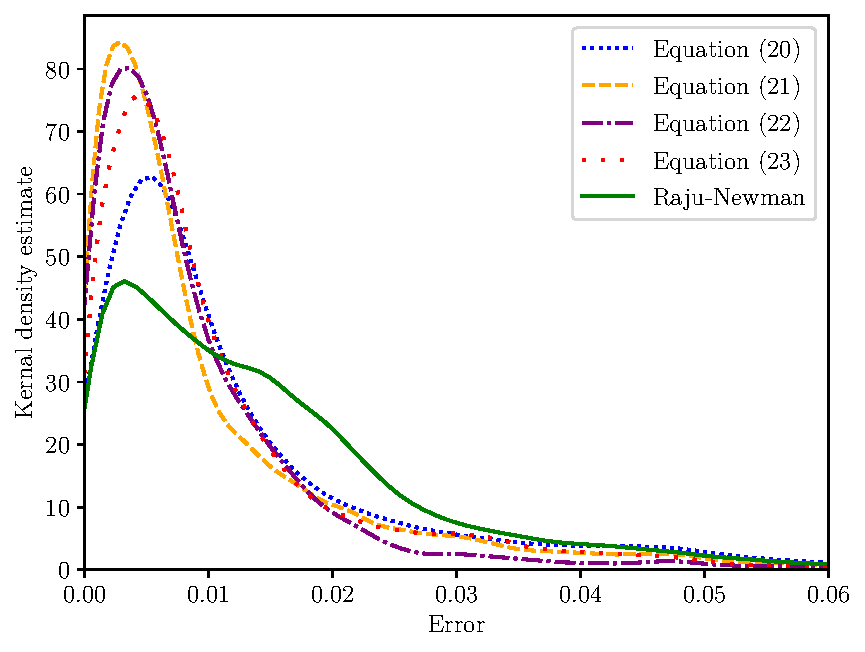
\includegraphics[width=0.45\textwidth]{Figures_pdf/kde.pdf} }}%
    \qquad
    \subfloat[\centering Parity plots]{{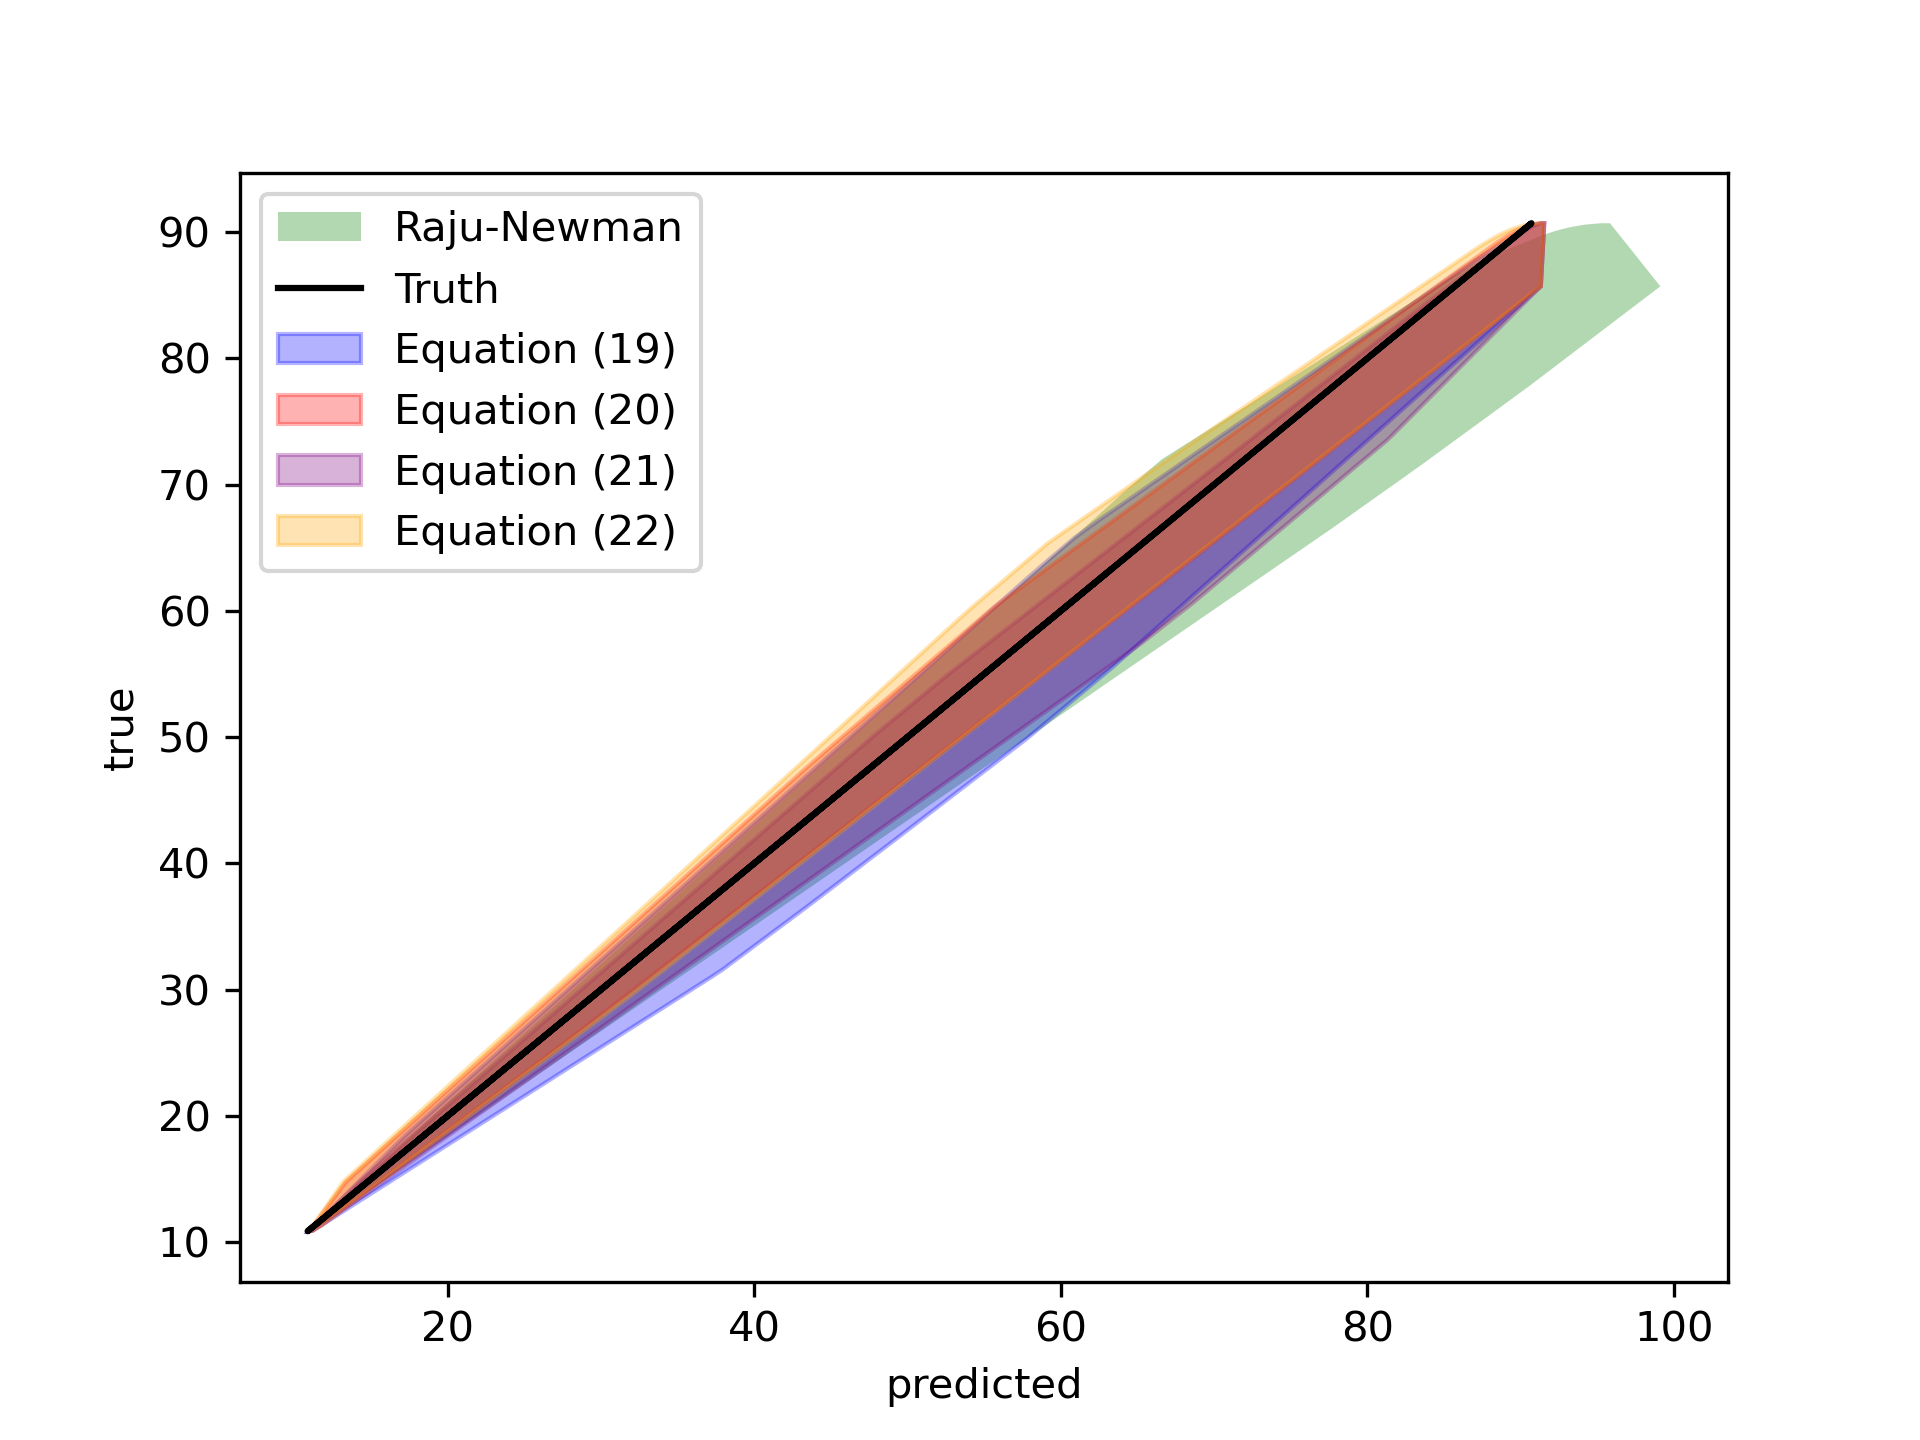
\includegraphics[width=0.45\textwidth]{Figures/parity_plot.png} }}%
    \caption{(a) Density plot for the errors of each of the equations. (b) Parity plot with each of the different equations.}%
    \label{fig:error_plots}%
\end{figure}

\begin{figure}
    \centering
    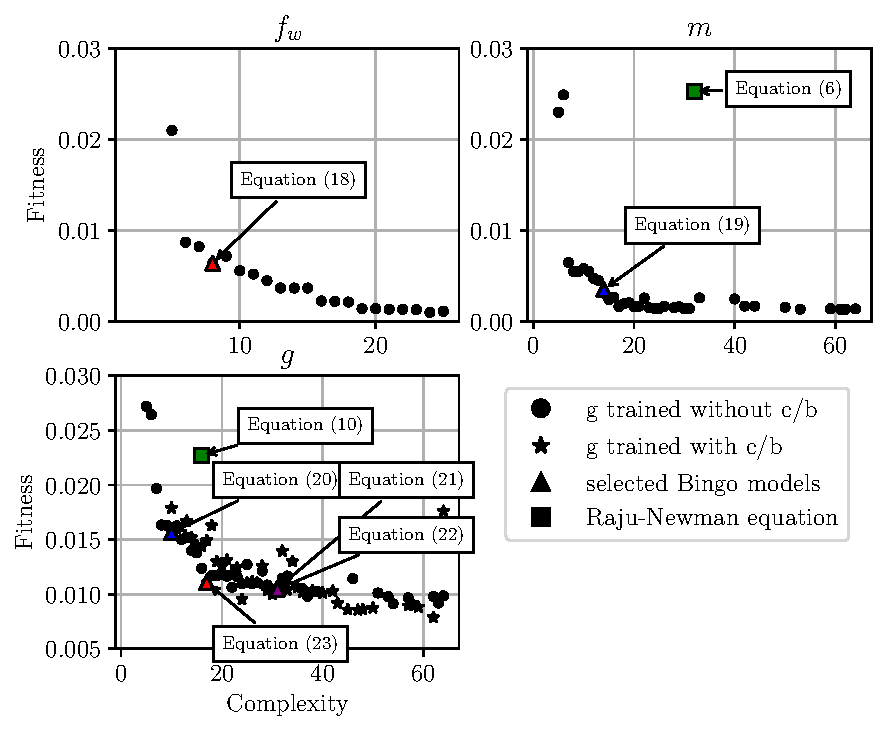
\includegraphics[width=\textwidth]{Figures_pdf/Pareto_fronts.pdf}
    \label{fig:perato_front}
    \caption{Pareto fronts for $f_w$, $M$, and $g$. $f_w$ and $M$ have the same equation for all four models. Both the Pareto fronts for $g$ with and without $c/b$ are shown} 
\end{figure}

\begin{figure}%
    \centering
    \subfloat[\centering Distributions of error]{{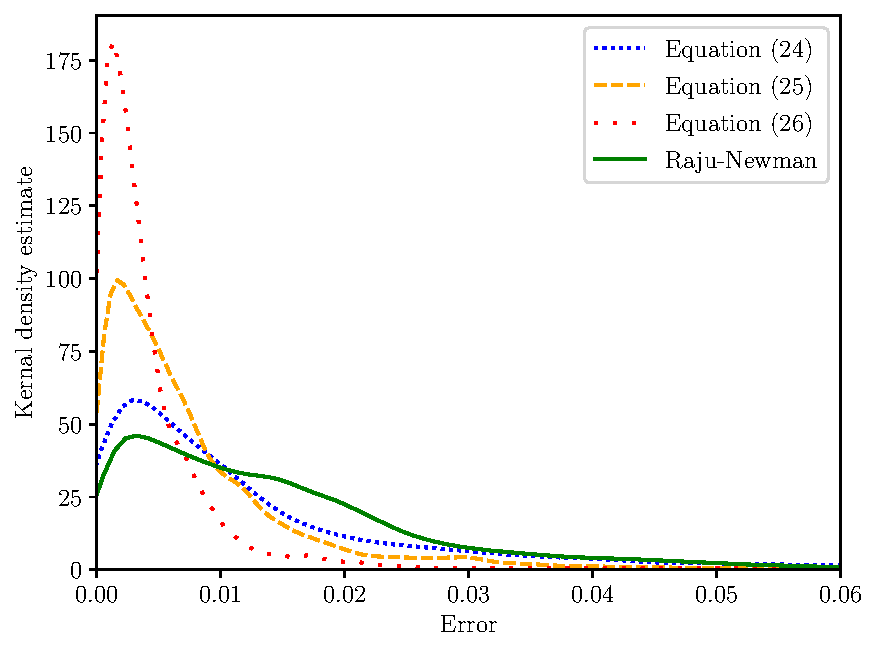
\includegraphics[width=0.45\textwidth]{Figures_pdf/kde_combo.pdf} }}%
    \qquad
    \subfloat[\centering Parity plots]{{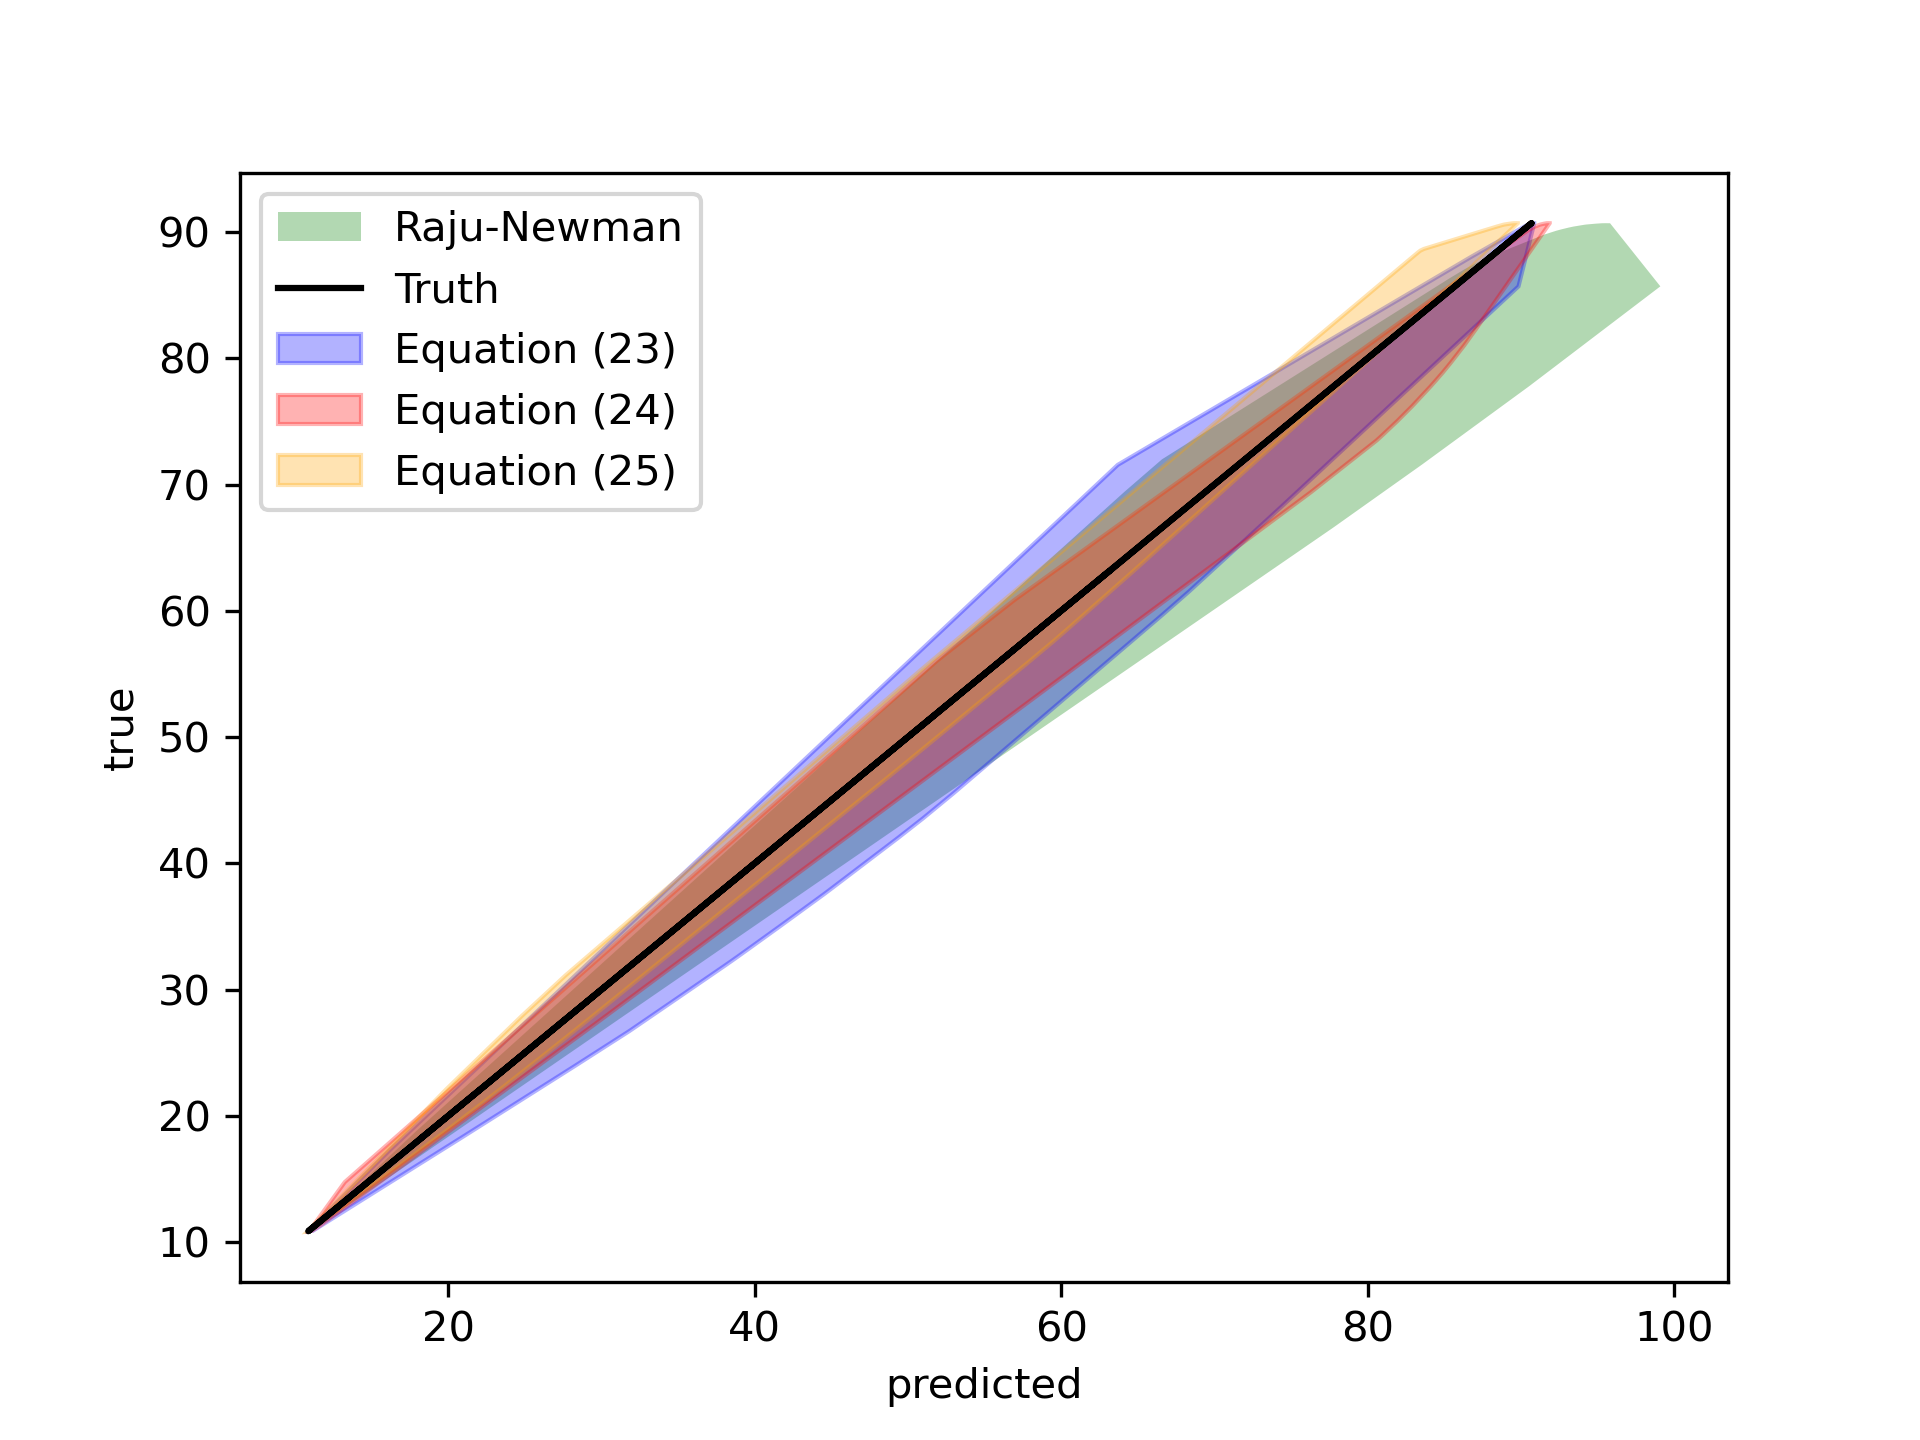
\includegraphics[width=0.45\textwidth]{Figures/parity_plot_everything.png} }}%
    \caption{(a) Density plot for the errors of each of the equations from the combined selection. (b) Parity plot with each of the different equations from the combined selection.}%
    \label{fig:combo_error_plots}%
\end{figure}


The Pareto front for the model selection using the Pareto front generated using all possible combinations of the models $f_w$, $M$, and $g$ can be seen in figure \ref{fig:perato_front_everything}. Equations [\ref{eqn:Bingo_matching_error_combo}-\ref{eqn:Bingo_optimal_combo}] are the equations gathered from the Pareto front of all possible equations. The error distributions and parity plots for these models can be seen in figure \ref{fig:combo_error_plots}.

\begin{equation} \label{eqn:Bingo_matching_error_combo}
    \begin{cases}
        f_w = 0.13 \frac{c}{b} + 0.13 \frac{a}{t} + 1.0
        \\
        M = - 0.223 \frac{a}{t} + 1 + \frac{0.223 \frac{a}{t}}{\frac{a}{c}}
        \\
        g = 0.554 \frac{a}{t} \left(1 - \sin^{0.491^{\frac{a}{c}}}{\left(\phi \right)}\right)
    \end{cases}
\end{equation}

\begin{equation} \label{eqn:Bingo_matching_complexity_combo}
    \begin{cases}
        f_w = \frac{- 63.94 \frac{c}{b} + 51.875 \frac{a}{t} + 38.855}{- 63.94 \frac{c}{b} + 43.336 \frac{a}{t} + 38.855}
        \\
        M = \frac{- 0.028 \frac{a}{c}^{3} + \frac{a}{c}^{2} \left(\frac{a}{c} + 0.028\right) - 0.644 \frac{a}{c} \frac{a}{t} \left(\frac{a}{c} \frac{a}{t} - 0.044\right) \left(- \frac{a}{c} \left(\frac{a}{t} - 1.103\right) + 0.044\right) + 0.644 \frac{a}{t} \left(\frac{a}{c} \frac{a}{t} - 0.044\right) \left(- \frac{a}{c} \left(\frac{a}{t} - 1.103\right) + 0.044\right)}{\frac{a}{c}^{3}}
        \\
        g = - \frac{0.127 \frac{a}{c} \left(\sin^{\frac{a}{t}}{\left(\phi \right)} - 1\right)}{\left(\cos{\left(\frac{c}{b} \right)} - 0.66\right) \left(\frac{a}{c}^{1.811} - 1.066 \frac{a}{t} + 0.992\right)}
    \end{cases}
\end{equation}

\begin{equation} \label{eqn:Bingo_optimal_combo}
    \begin{cases}
        f_w = - \frac{a}{t} \left(\left(1.216 \frac{c}{b}^{2} + 0.11\right) \left(\frac{a}{t} - \sqrt{- \frac{c}{b}^{2} - 0.751}\right) - 0.119\right) + 1.0
        \\
        M = \frac{a}{c}^{\frac{- 0.037 \frac{a}{c} - 0.046 \frac{a}{t} \left(\frac{a}{c}^{2} - 15.413\right) \left(\frac{a}{t} - 1.114\right) \left(1.919 \frac{a}{t} - 0.489\right) - 0.06}{\frac{a}{c} + 0.599}}
        \\
        g = - \frac{1.232 \left(\frac{a}{c} \left(\frac{a}{c} + 0.06\right) \left(0.103 \left(1 - \sin{\left(\phi \right)}\right)^{\frac{3}{2}} + 0.017\right) - 0.36 \left(\frac{a}{t} - 0.187\right) \left(\frac{a}{c} \left(\left(\frac{a}{c} + 0.06\right) \left(0.017 \frac{a}{c} + 0.033 \frac{a}{t} - 0.409 \frac{c}{b}^{2} \right) - 0.646\right) \left(\frac{a}{c} + 2 \frac{a}{t} \right) + 2.501 \frac{a}{c} + 0.1501\right)\right) \left(\sin{\left(\phi \right)} - 1\right)}{\frac{a}{c} \left(\frac{a}{c} + 0.06\right)}
    \end{cases}
\end{equation}


\begin{figure}
    \centering
    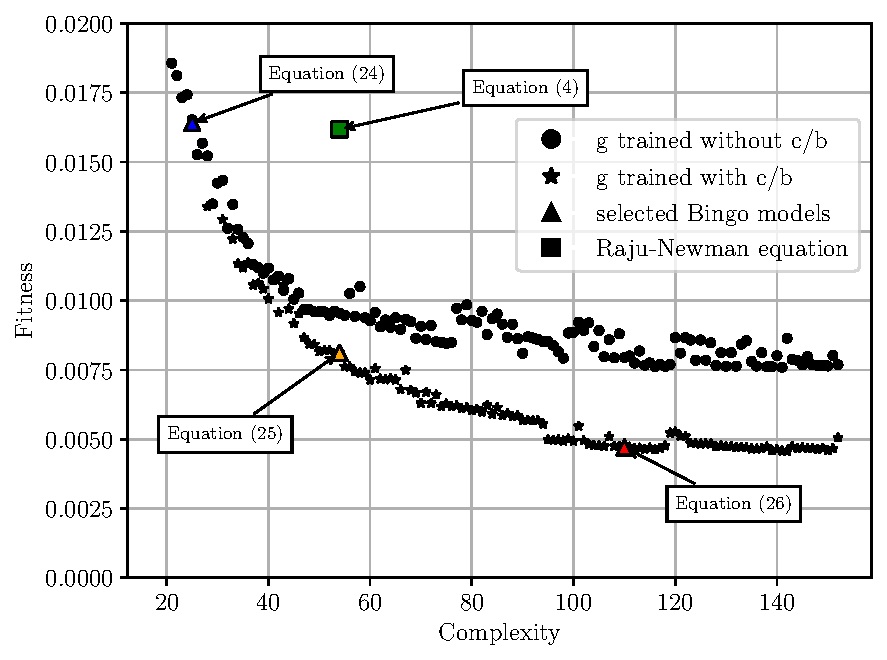
\includegraphics[width=\textwidth]{Figures_pdf/Pareto_fronts_combo.pdf}
    \label{fig:perato_front_everything}
    \caption{Pareto front for the models selected using all possible combinations.}
\end{figure}


Finally figure \ref{fig:perato_front_everything} shows all eight models on the same Pareto front. 

\begin{figure}
    \centering
    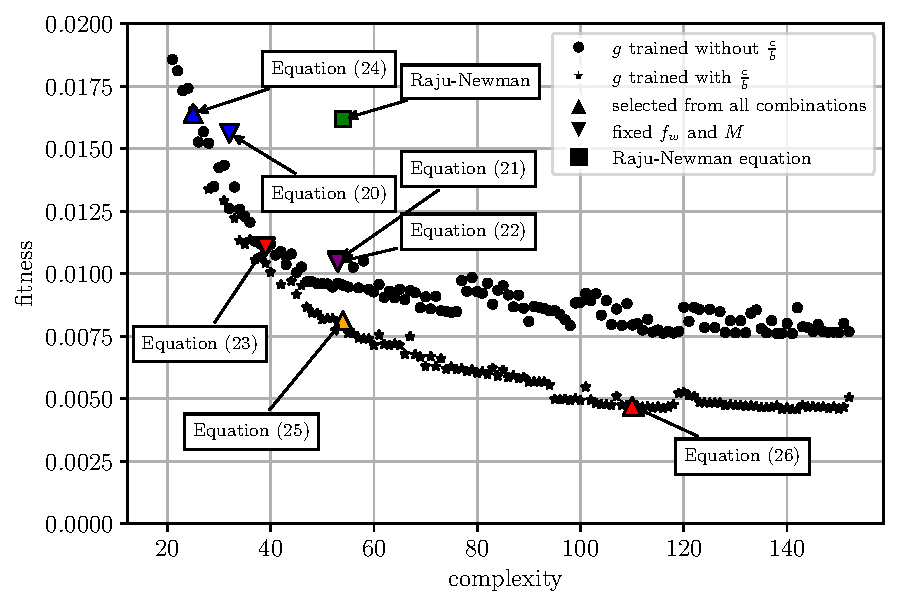
\includegraphics[width=\textwidth]{Figures_pdf/Pareto_fronts_everything.pdf}
    \label{fig:perato_front_everythin}
    \caption{Pareto front with all models the triangle markers correspond to the models that were individually selected and the square markers are the models selected using all possible combinations.}
\end{figure}

\begin{figure}
    \centering
    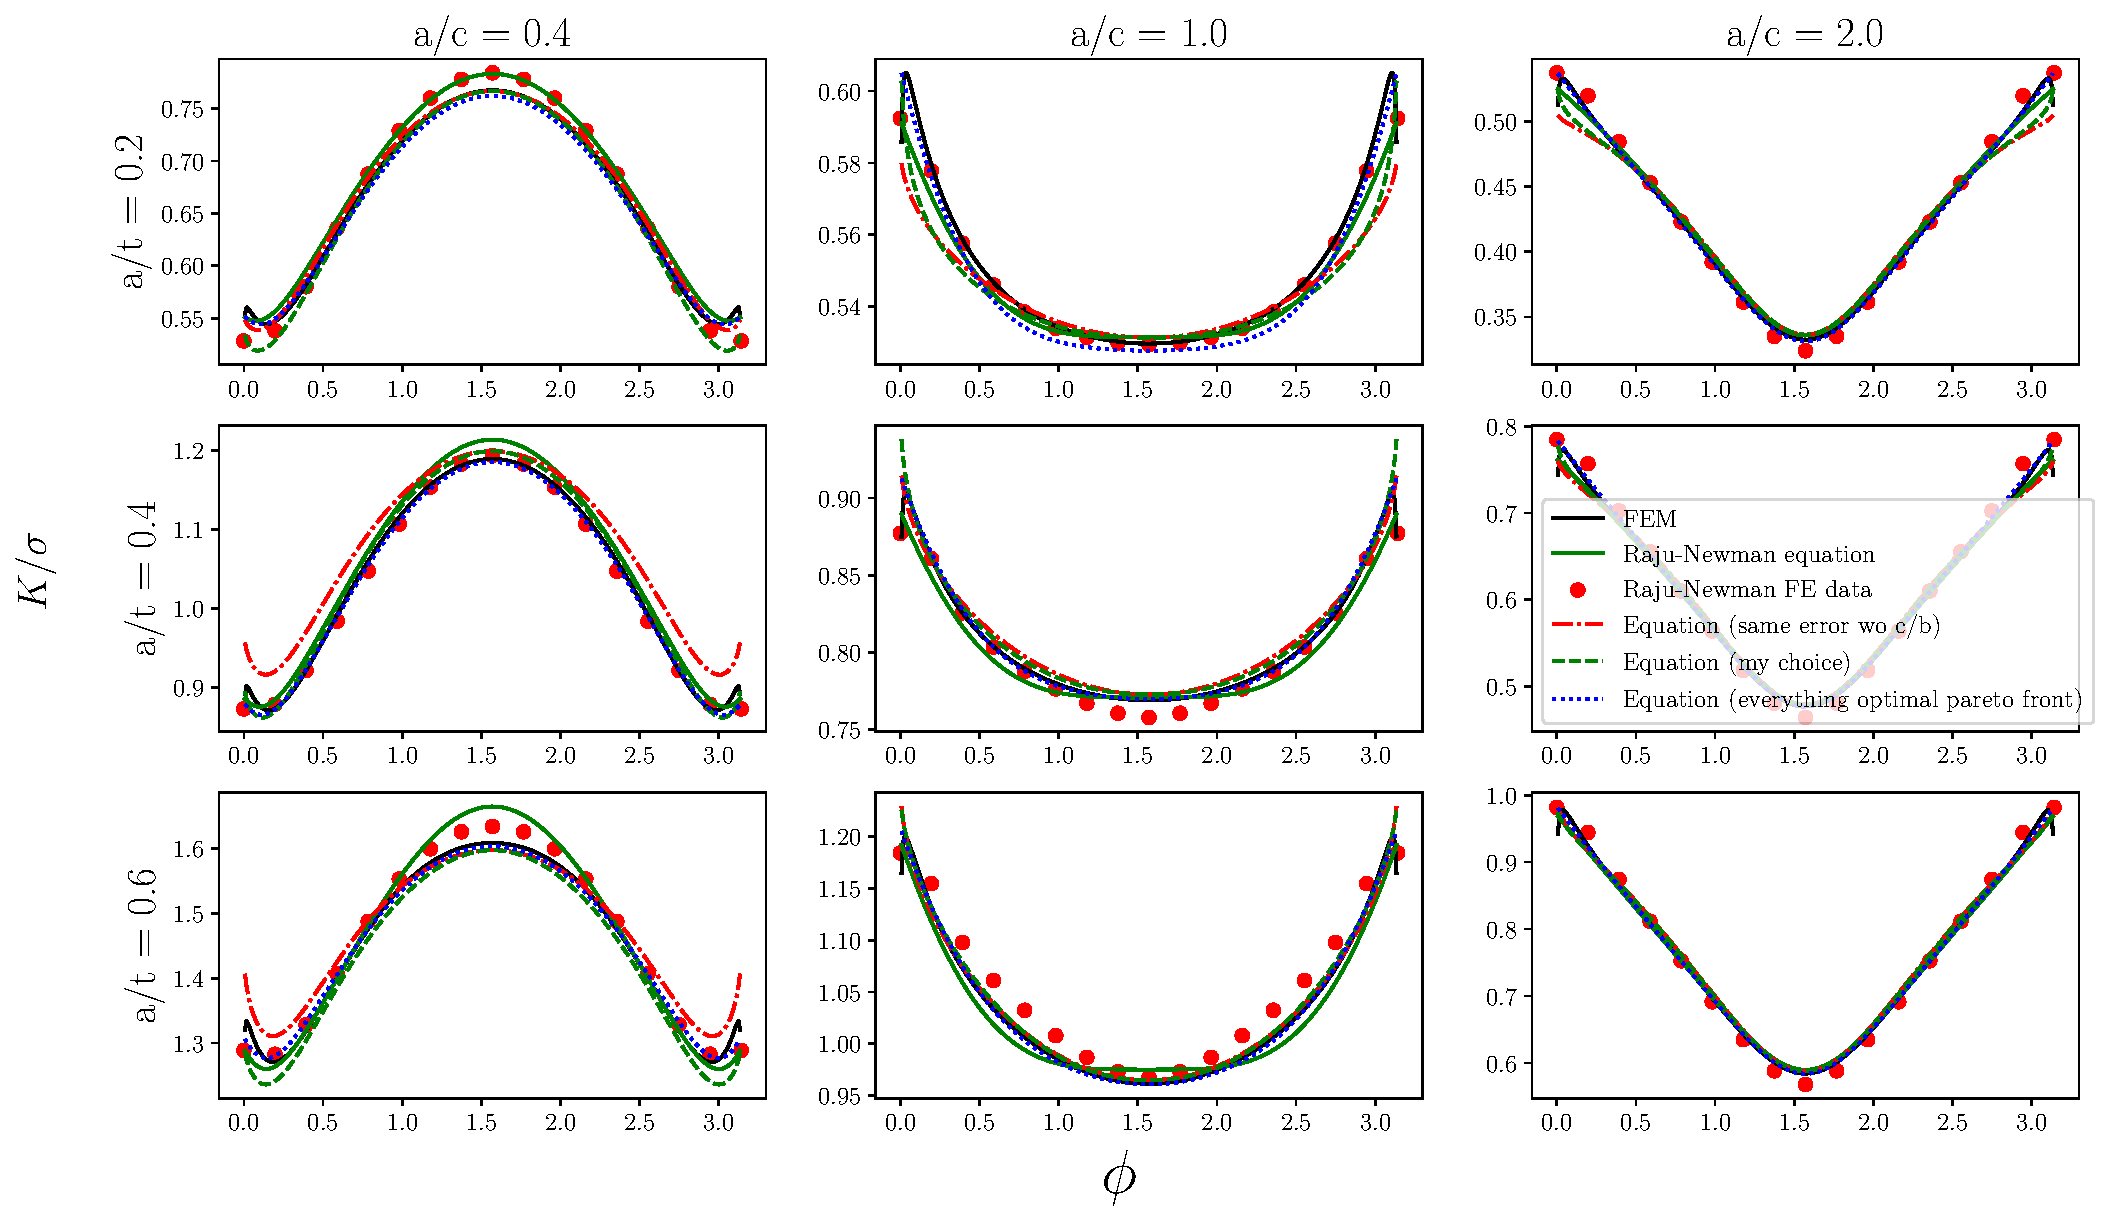
\includegraphics[width=\textwidth]{Figures_pdf/K_data_with_bingo.pdf}
    \label{fig:K_data_with_bingo}
    \caption{A sample of models comparing the SIFs collected from FRANC3D with the bingo equation, the Raju-Newman equation, and the Raju-Newman FE data.}
\end{figure}